\documentclass[12pt,dvipsnames,enabledeprecatedfontcommands]{scrartcl}
\usepackage{lmodern}
\usepackage{amssymb,amsmath}
\usepackage{ifxetex,ifluatex}
\usepackage{fixltx2e} % provides \textsubscript
\ifnum 0\ifxetex 1\fi\ifluatex 1\fi=0 % if pdftex
  \usepackage[T1]{fontenc}
  \usepackage[utf8]{inputenc}
\else % if luatex or xelatex
  \ifxetex
    \usepackage{mathspec}
  \else
    \usepackage{fontspec}
  \fi
  \defaultfontfeatures{Ligatures=TeX,Scale=MatchLowercase}
\fi
% use upquote if available, for straight quotes in verbatim environments
\IfFileExists{upquote.sty}{\usepackage{upquote}}{}
% use microtype if available
\IfFileExists{microtype.sty}{%
\usepackage[]{microtype}
\UseMicrotypeSet[protrusion]{basicmath} % disable protrusion for tt fonts
}{}
\PassOptionsToPackage{hyphens}{url} % url is loaded by hyperref
\usepackage[unicode=true]{hyperref}
\PassOptionsToPackage{usenames,dvipsnames}{color} % color is loaded by hyperref
\hypersetup{
            colorlinks=true,
            linkcolor=Maroon,
            citecolor=Blue,
            urlcolor=blue,
            breaklinks=true}
\urlstyle{same}  % don't use monospace font for urls
\usepackage{graphicx,grffile}
\makeatletter
\def\maxwidth{\ifdim\Gin@nat@width>\linewidth\linewidth\else\Gin@nat@width\fi}
\def\maxheight{\ifdim\Gin@nat@height>\textheight\textheight\else\Gin@nat@height\fi}
\makeatother
% Scale images if necessary, so that they will not overflow the page
% margins by default, and it is still possible to overwrite the defaults
% using explicit options in \includegraphics[width, height, ...]{}
\setkeys{Gin}{width=\maxwidth,height=\maxheight,keepaspectratio}
\IfFileExists{parskip.sty}{%
\usepackage{parskip}
}{% else
\setlength{\parindent}{0pt}
\setlength{\parskip}{6pt plus 2pt minus 1pt}
}
\setlength{\emergencystretch}{3em}  % prevent overfull lines
\providecommand{\tightlist}{%
  \setlength{\itemsep}{0pt}\setlength{\parskip}{0pt}}
\setcounter{secnumdepth}{5}
% Redefines (sub)paragraphs to behave more like sections
\ifx\paragraph\undefined\else
\let\oldparagraph\paragraph
\renewcommand{\paragraph}[1]{\oldparagraph{#1}\mbox{}}
\fi
\ifx\subparagraph\undefined\else
\let\oldsubparagraph\subparagraph
\renewcommand{\subparagraph}[1]{\oldsubparagraph{#1}\mbox{}}
\fi

% set default figure placement to htbp
\makeatletter
\def\fps@figure{htbp}
\makeatother

%\documentclass{article}

% %packages
 \usepackage{booktabs}

\usepackage{multirow}
\usepackage{multicol}

\usepackage{graphicx}
\usepackage{longtable}
\usepackage{ragged2e}
\usepackage{etex}
%\usepackage{yfonts}
\usepackage{marvosym}
\usepackage[notextcomp]{kpfonts}
\usepackage{nicefrac}
\newcommand*{\QED}{\hfill \footnotesize {\sc Q.e.d.}}
\usepackage{floatrow}



\usepackage[textsize=scriptsize, textwidth = 1.5cm]{todonotes}
%\linespread{1.5}


\setlength{\parindent}{10pt}
\setlength{\parskip}{1pt}


%language
\usepackage{times}
\usepackage{t1enc}
%\usepackage[utf8x]{inputenc}
%\usepackage[polish]{babel}
%\usepackage{polski}

\usepackage{mathptmx}
\usepackage[scaled=0.88]{helvet}


%AMS
\usepackage{amsfonts}
\usepackage{amssymb}
\usepackage{amsthm}
\usepackage{amsmath}
\usepackage{mathtools}

\usepackage{geometry}
 \geometry{a4paper,left=20mm,top=15mm,bottom = 20mm, right = 20mm}


%environments
\newtheorem{fact}{Fact}



%abbreviations
\newcommand{\ra}{\rangle}
\newcommand{\la}{\langle}
\newcommand{\n}{\neg}
\newcommand{\et}{\wedge}
\newcommand{\jt}{\rightarrow}
\newcommand{\ko}[1]{\forall  #1\,}
\newcommand{\ro}{\leftrightarrow}
\newcommand{\exi}[1]{\exists\, {_{#1}}}
\newcommand{\pr}[1]{\mathsf{P}(#1)}
\newcommand{\cost}{\mathsf{cost}}


\newcommand{\odds}{\mathsf{Odds}}
\newcommand{\ind}{\mathsf{Ind}}
\newcommand{\nf}[2]{\nicefrac{#1\,}{#2}}
\newcommand{\R}[1]{\texttt{#1}}
\newcommand{\prr}[1]{\mbox{$\mathtt{P}_{prior}(#1)$}}
\newcommand{\prp}[1]{\mbox{$\mathtt{P}_{posterior}(#1)$}}



\newtheorem{q}{\color{blue}Question}
\newtheorem{lemma}{Lemma}
\newtheorem{theorem}{Theorem}



%technical intermezzo
%---------------------

\newcommand{\intermezzoa}{
	\begin{minipage}[c]{13cm}
	\begin{center}\rule{10cm}{0.4pt}



	\tiny{\sc Optional Content Starts}
	
	\vspace{-1mm}
	
	\rule{10cm}{0.4pt}\end{center}
	\end{minipage}\nopagebreak 
	}


\newcommand{\intermezzob}{\nopagebreak 
	\begin{minipage}[c]{13cm}
	\begin{center}\rule{10cm}{0.4pt}

	\tiny{\sc Optional Content Ends}
	
	\vspace{-1mm}
	
	\rule{10cm}{0.4pt}\end{center}
	\end{minipage}
	}
%--------------------

\DeclareUnicodeCharacter{0301}{*************************************}




















\newtheorem*{reply*}{Reply}
\usepackage{enumitem}
\newcommand{\question}[1]{\begin{enumerate}[resume,leftmargin=0cm,labelsep=0cm,align=left]
\item #1
\end{enumerate}}

\usepackage{float}

% \setbeamertemplate{blocks}[rounded][shadow=true]
% \setbeamertemplate{itemize items}[ball]
% \AtBeginPart{}
% \AtBeginSection{}
% \AtBeginSubsection{}
% \AtBeginSubsubsection{}
% \setlength{\emergencystretch}{0em}
% \setlength{\parskip}{0pt}






\usepackage[authoryear]{natbib}

%\bibliographystyle{apalike}
\usepackage{booktabs}
\usepackage{longtable}
\usepackage{array}
\usepackage{multirow}
\usepackage{wrapfig}
\usepackage{float}
\usepackage{colortbl}
\usepackage{pdflscape}
\usepackage{tabu}
\usepackage{threeparttable}
\usepackage{threeparttablex}
\usepackage[normalem]{ulem}
\usepackage{makecell}
\usepackage{xcolor}

\author{}
\date{\vspace{-2.5em}}

\begin{document}

\begin{center}
\Large \textbf{A bayesian method of cosine-based word2vec bias estimation}
\end{center}

\vspace{1mm}

A considerable amount of literature exists on bias detection and
mitigation in NLP models, especially word2vec embeddings, which
represent words as number vectors (see e.g. {[}1{]} and {[}4{]} and
references therein). The most common method used compares cosine
similarity between words from protected groups and attributes that are
considered to be stereotypical or harmful in some way, and this method
will be in our focus.

In one well-known approach, {[}2{]} proposed the Word Embedding
Association Test (WEAT). The idea is that the measure of biases between
two sets of target words, \(X\) and \(Y\), (we call them protected
words) should be quantified in terms of the cosine similarity between
the protected words and attribute words coming from two sets of
stereotype attribute words, \(A\) and \(B\) (we'll call them
attributes). For instance, \(X\) might be a set of male names, \(Y\) a
set of female names, \(A\) might contain stereotypically male-related
career words, and \(B\) stereotypically female-related family words.
WEAT is a modification of the Implicit Association Test (IAT) {[}7{]}
used in psychology and uses almost the same word sets, allowing for a
\emph{prima facie} sensible comparison with bias in humans. The
association difference for a term \(t\) is \(s(t,A,B)\), and the effect
size is computed by normalizing the difference in means as follows:

\vspace{-3mm}

\footnotesize 

\begin{align}
\mathsf{s}(t,A,B)  = \frac{\sum_{a\in A}f(t,a)}{\vert A\vert} - \frac{\sum_{b\in B}f(t,b)}{\vert B\vert}
& \,\,\,\,\,\,\,\,\,\,\,\,\,\,\,\,\,
\mathsf{bias}(A,B)  = \frac{
\mu(\{s(x,A,B)\}_{x\in X}) -\mu(\{s(y,A,B)\}_{y\in Y}) 
}{
\sigma(\{s(w,A,B)\}_{w\in X\cup Y})
} \tag{WEAT}
\end{align}

\normalsize
\noindent {[}2{]} show that significant biases---thus measured---
similar to the ones discovered by IAT can be discovered in word
embeddings. {[}5{]} extends the methodology to a multilingual and
cross-lingual setting; a similar methodology is employed by {[}3{]}, who
employ word embeddings trained on corpora from different decades.
{[}6{]} modify WEAT to a multi-class setting, introducing Mean Average
Cosine (MAC) similarity as a measure of bias (in fact, in the paper they
report distances rather than similarities). Let
\(T = \{t_1, \dots, t_k\}\) be a class of protected word embeddings, and
let each \(A_j\in A\) be a set of attributes stereotypically associated
with a protected word). Then:

\vspace{-2mm}

\footnotesize

\begin{align}
\mathsf{S}(t_i, A_j)  = \frac{1}{\vert A_j\vert}\sum_{a\in A_j}\mathsf{cos}(t,a) & \,\,\,\,\,\,\,\,\,\,\,\,\,\,\,\,\,\,\,\,\,\,\,\,\,
\mathsf{MAC}(T,A)  = \frac{1}{\vert T \vert \,\vert A\vert}\sum_{t_i \in T }\sum_{A_j \in A} S(t_i,A_j) \tag{MAC}
\end{align}

\normalsize  \noindent That is, for each protected word and each
attribute class, they first take the mean for this protected word and
all attributes in a given attribute class, and then take the mean of
thus obtained means for all the protected words.

Such methods are statistically problematic. One issue, specific to
{[}6{]}, is that no distinction is made based on whether given a
protected word and a class of attributes is stereotypically associated
with this protected word or a different protected word. A related,
general problem, is that all the authors ignore the step of comparing
their results with control groups, especially control groups of
stereotype-neutral human attributes. That such a move is important is
suggested for instance by Figure 1 prepared using the original word list
for religion-related protected words extended with control attributes,
where such human attributes are also closer to protected classes than 1.

Another, also serious problem, is that all the authors calculate means
of means and their authors run statistical tests on sets of means.
Unforutnately, by pre-averaging the data they throw away information
about sample sizes, and they remove variation, and so pre-averaging
tends to manufacture false confidence.

All such approaches come up with rather short lists of protected words
and rather short lists of stereotypical attributes. Clearly, these are
not complete list. So let's treat them as samples from richer pools of
stereotypical predicates and let's take the uncertainty and variation
involved seriously. To illustrate, let's employ the formulas used by
{[}2{]} in a simple simulation.

\noindent

\begin{tabular}{ll}
\begin{minipage}[c]{0.35\linewidth}
\scalebox{0.65}{
\begin{tabular}{cccccc}\toprule
$X$ to $A$  & $X$ to $B$ & $Y$ to $A$ & $Y$ to $B$ & $\sigma$  & WEAT \\
\midrule
0 & 0 & 0 & 0 & 0.05 & 1.82 \\
0 & 0 & 0 & 0 & 0.001 & -1.93\\
.1 & 0 & 0 & .1 & 0.05 & 1.49 \\
.1 & 0 & 0 & .1 & .1 & 1.22\\
\bottomrule
\end{tabular}
}
\end{minipage}& \begin{minipage}[c]{0.6\linewidth}
Two protected classes, $X=\{t_1,t_2\}$ and $Y=\{t_3,t_4\}$, and two five-element attribute sets $A$ and $B$. One simple simulation draws normally distributed values for such combinations for two cases in which the underlying mean similarities are in fact equal, two cases in which they are different, and the underlying variances are different (code available upon request).
\end{minipage}
\end{tabular}

\vspace{1mm}

The following observations are worthwhile. (1) For points randomly drawn
from distributions where there is no difference in means the calculated
effect size can easily be 1.82, whereas the largest effect size reported
by {[}2{]} is 1.81. (2) For samples from distributions where the means
are different, the (absolute) effect sizes can easily be lower than in
the first two simulations. As Figure 2. illustrates, quite some
uncertainty is involved, far from what systematically low mean-based
p-values reported in the papers might suggest. Part of the problem is
random variation unaccounted for in the original approach (see Figures 3
and 4 for an example), and part of the problem is that that
non-negligible changes in effect size can result from a shift in the
standard deviation of the original process, because with the decrease of
standard deviation the numerator in (WEAT) decreases.

To improve on the situation, we build bayesian models to estimate the
biases involved using the raw datapoints, actually using control groups,
distinguishing the connection types, and taking the uncertainty involved
seriously. For the general impact of being associated, we build models
using STAN according to the following specification:

\footnotesize 

\vspace{-5mm}

\begin{align}
cosineDistance_i  & \sim dnorm(\mu_i, \sigma) \\
\mu_i & = m_{pw} + co_{con}\\
m_{pw} & \sim dnorm(1,.5) \\
co_{con} & \sim dnorm(0,1) \\
\sigma &\sim  dcauchy(0,1)
\end{align}

\normalsize 

The resulting coefficients for the religion dataset based on Reddit
embeddings are in Figure 5. While there is some difference in the means,
the 89\% highest posterior density invervals are quite wide and include
0s for all the coefficients. Then, motivated by large differences
between the status of different protected words, we build bayesian
models with separate mean estimates, with the same regularizing priors
as before. The results for the religion dataset based on Reddit
embeddings are in Figure 6.

We build analogous models for other topic groups (race, gender), and
different embeddings (Google, and hard-debiased Reddit). The general
conclusion is that once we proceed this way, the situation is much less
obvious. The word list sizes are small, sample sizes are small, and so
posterior density intervals are wide. Some stronger bias can be
discerned in the gender case. Moreover, sometimes the difference between
associated, different and human, are not very impressive. The cost of
debiasing turns out sometimes to be that neutral human predicates get
closer to protected classes (in religion), change in gender after
debiasing is really minor with zero still out out of HPDI range, and
debiasing improvement for race is a small improvement achieved at the
price of moving neutral terms closer to protected words (there is no
space to visualise these results in this abstract).

The bottom line is that if we want to take bias seriously, so should we
approach the uncertainty involved in our estimations. There is no
replacement for proper statistical evaluation that does not discard
information about the uncertaintly involved, larger word lists are
needed, and visualisation of the results particular protected classes
provides much better guidance than chasing a single metric based on a
means of means.

\pagebreak

\begin{center}
\begin{figure}[!htb]\centering
   \begin{minipage}{0.48\textwidth}

\begin{center}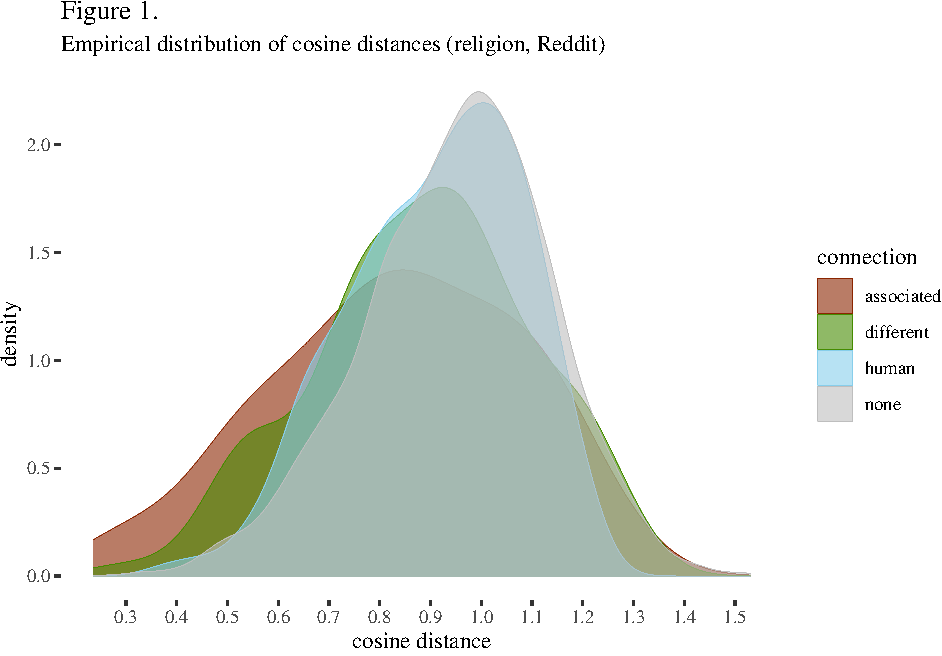
\includegraphics[width=1\linewidth]{abstractESSLLI1_files/figure-latex/unnamed-chunk-1-1} \end{center}
   \end{minipage}
   \begin {minipage}{0.48\textwidth}

\begin{center}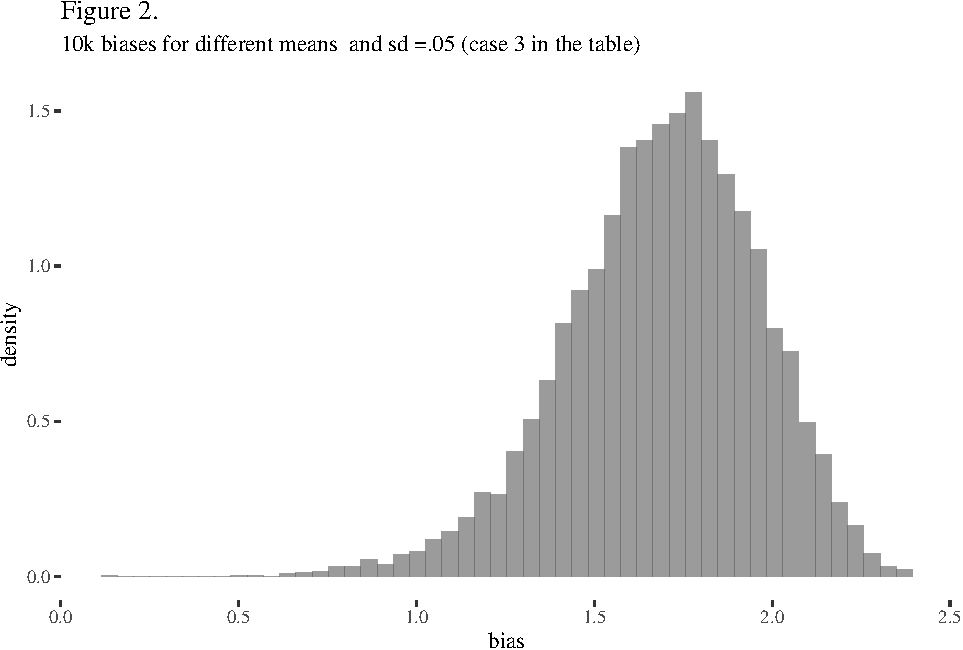
\includegraphics[width=1\linewidth]{abstractESSLLI1_files/figure-latex/unnamed-chunk-2-1} \end{center}
   \end{minipage}
   
   
  \begin{minipage}{0.48\textwidth}

\begin{center}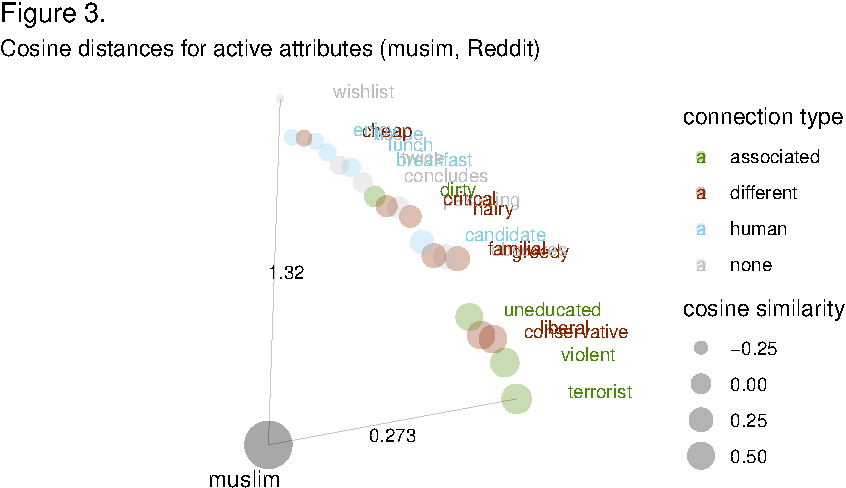
\includegraphics[width=1\linewidth]{abstractESSLLI1_files/figure-latex/unnamed-chunk-3-1} \end{center}
\end{minipage}
   \begin {minipage}{0.48\textwidth}

\begin{center}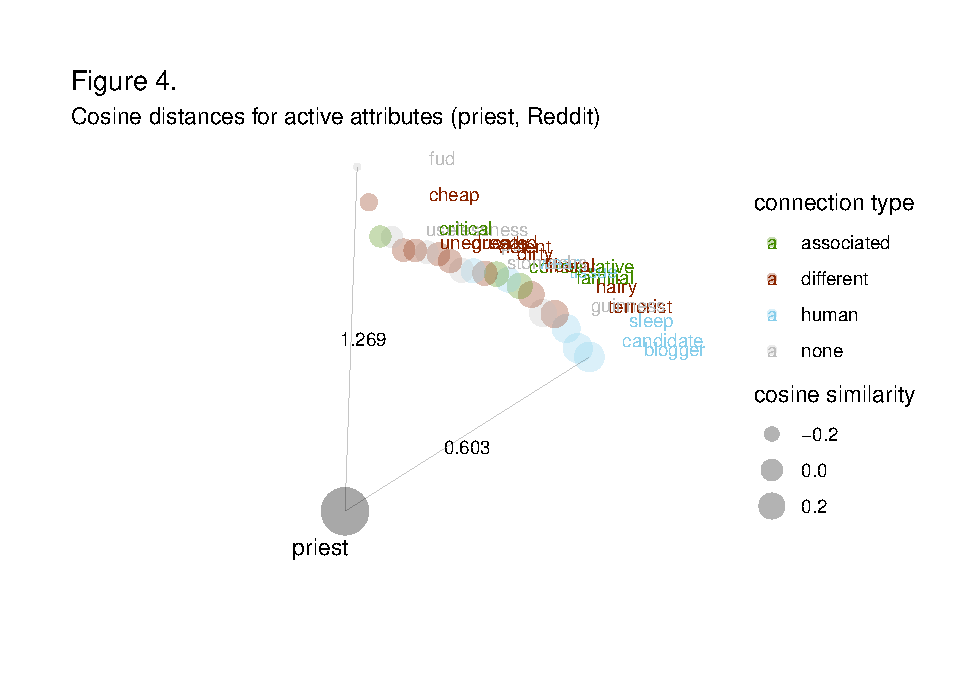
\includegraphics[width=1\linewidth]{abstractESSLLI1_files/figure-latex/unnamed-chunk-4-1} \end{center}
   \end{minipage}
   
   
   
   
  \begin{minipage}{0.38\textwidth}
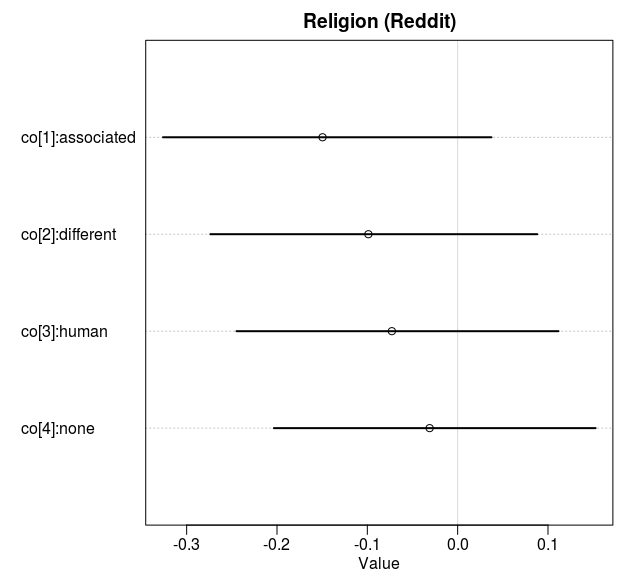
\includegraphics[width=7cm]{../images/religionCoeffs.jpeg}
\end{minipage}
   \begin {minipage}{0.58\textwidth}
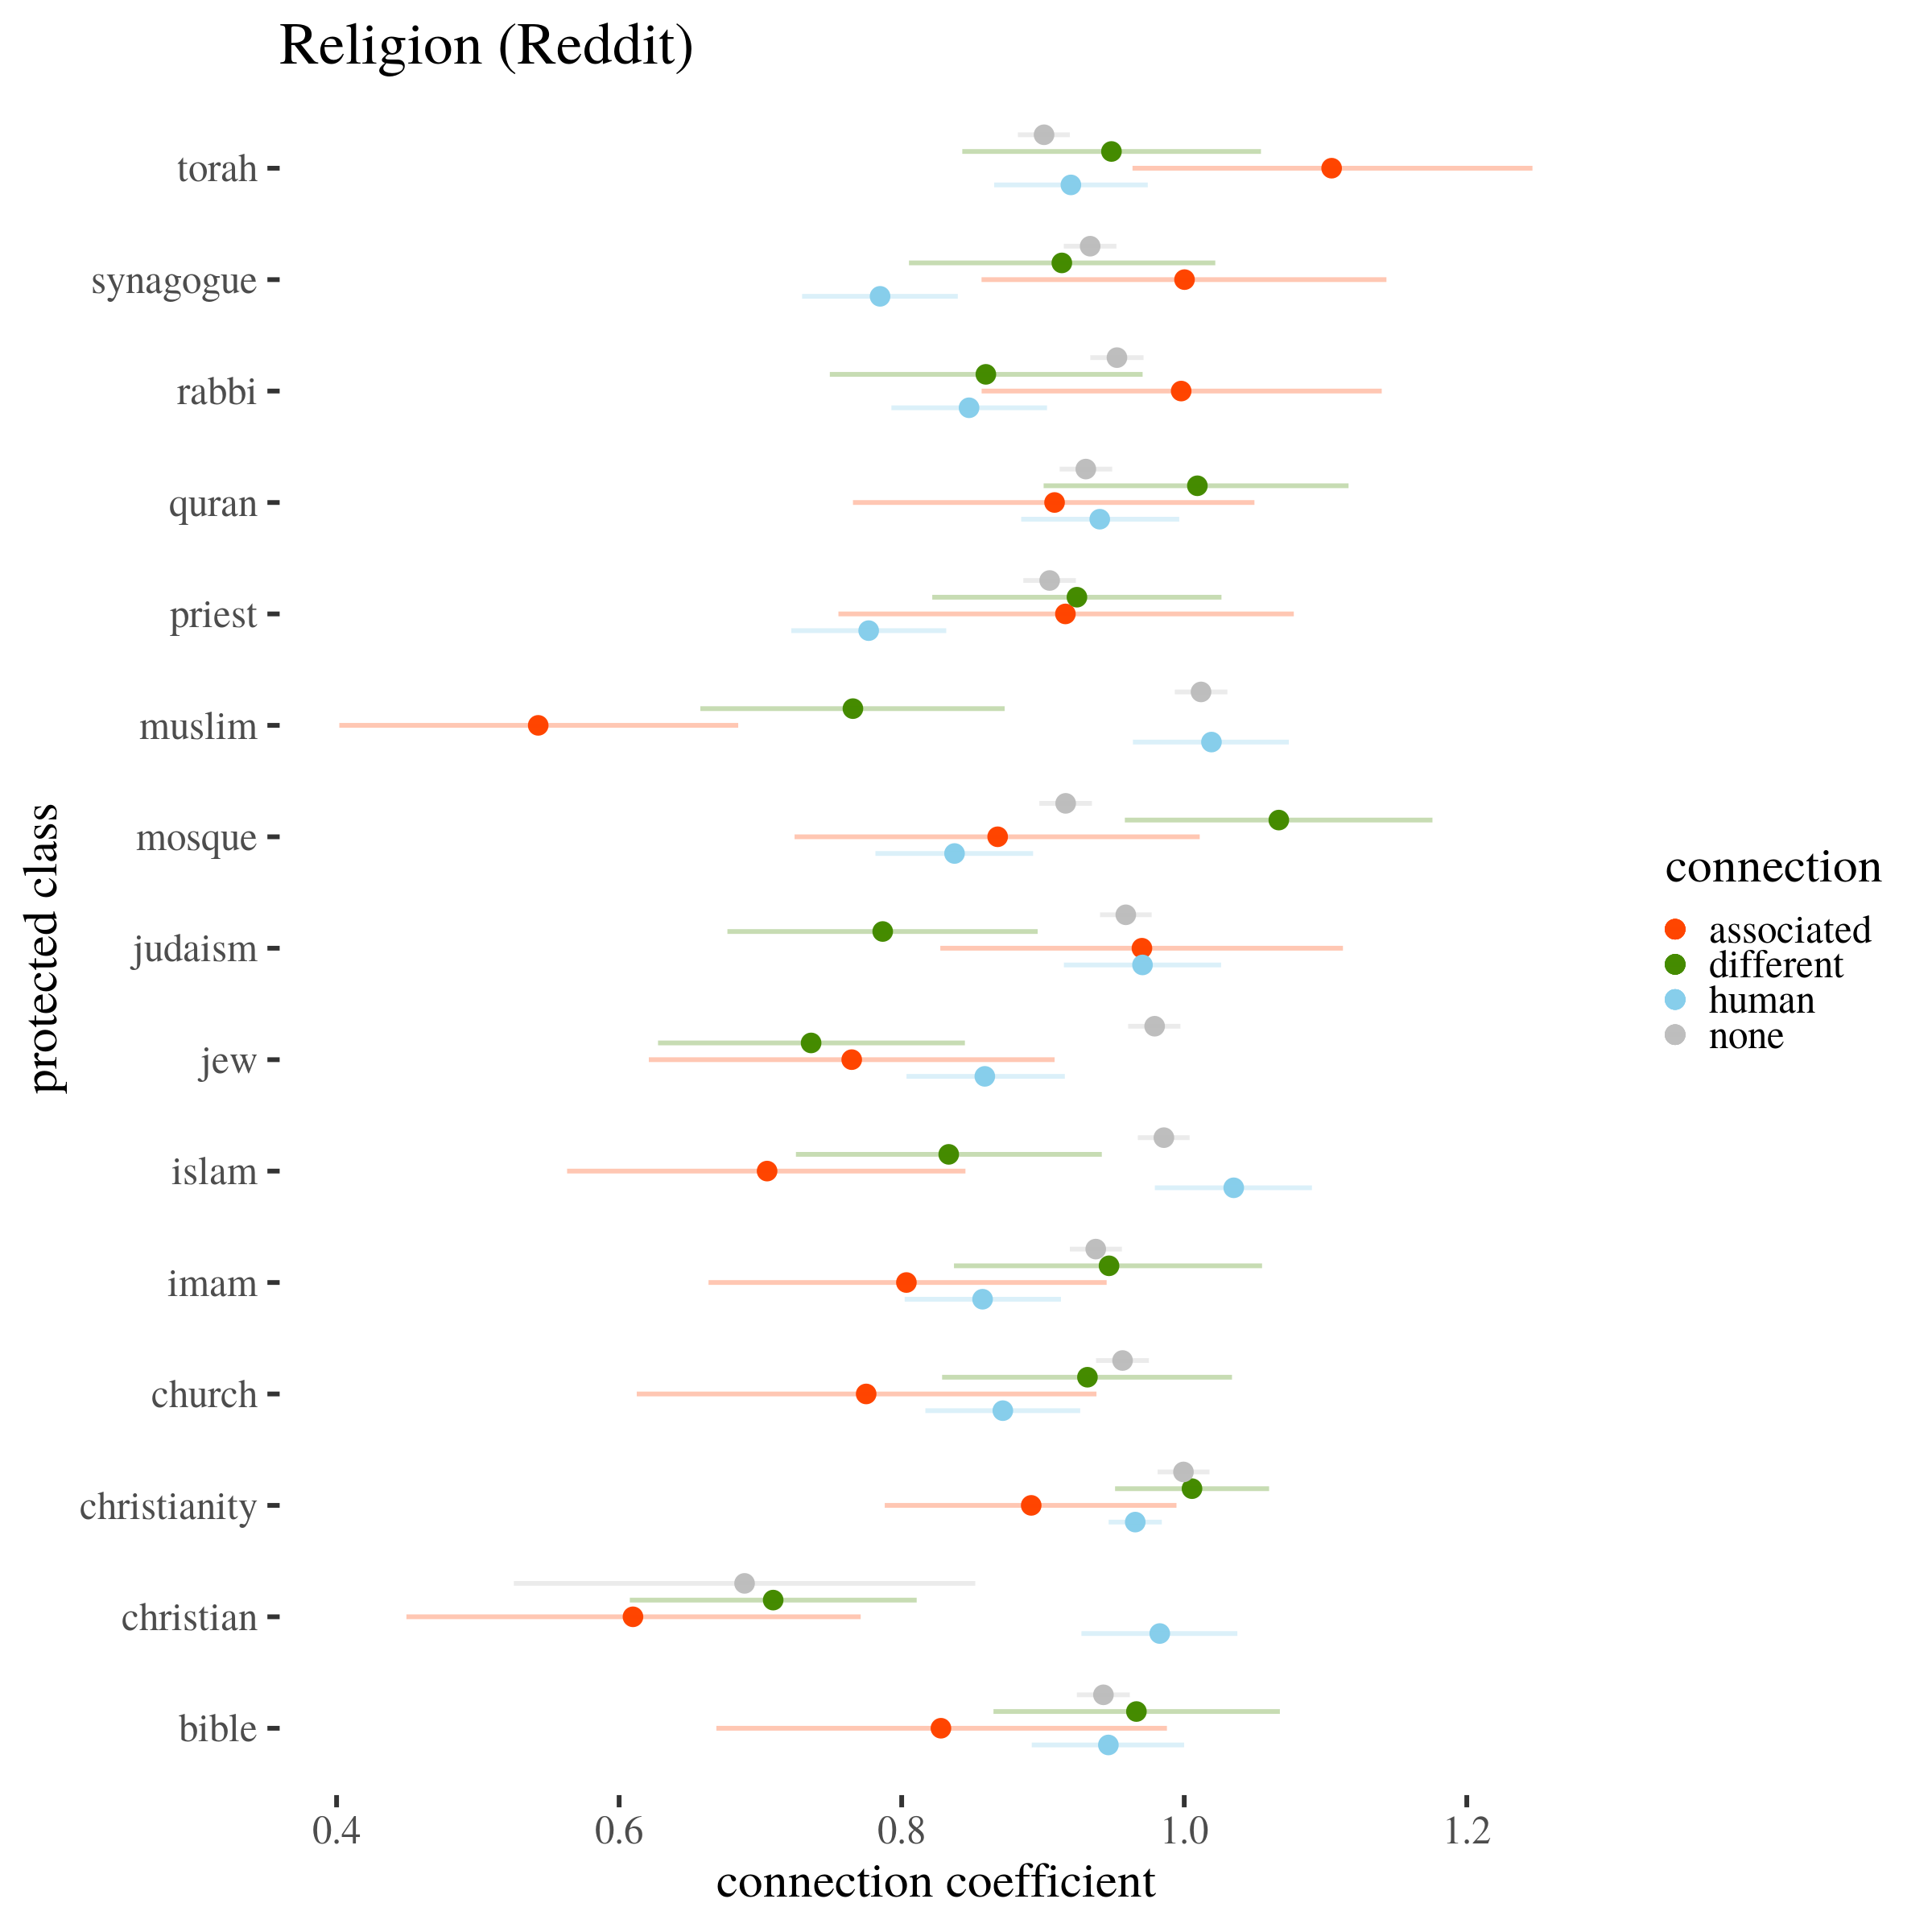
\includegraphics{../images/visReligionReddit.png}
   \end{minipage}
\end{figure}


\end{center}

\scriptsize 

\vspace{-4mm}

\hypertarget{refs}{}
\hypertarget{ref-bolukbasi2016man}{}
{[}1{]} Tolga Bolukbasi, Kai-Wei Chang, James Zou, Venkatesh Saligrama,
and Adam Kalai. 2016. Man is to computer programmer as woman is to
homemaker? Debiasing word embeddings.

\hypertarget{ref-Caliskan2017semanticsBiases}{}
{[}2{]} Aylin Caliskan, Joanna J. Bryson, and Arvind Narayanan. 2017.
Semantics derived automatically from language corpora contain human-like
biases. \emph{Science} 356, 6334 (April 2017), 183--186.
DOI:\url{https://doi.org/10.1126/science.aal4230}

\hypertarget{ref-Garg2018years}{}
{[}3{]} Nikhil Garg, Londa Schiebinger, Dan Jurafsky, and James Zou.
2018. Word embeddings quantify 100 years of gender and ethnic
stereotypes. \emph{Proceedings of the National Academy of Sciences} 115,
16 (April 2018), E3635--E3644.
DOI:\url{https://doi.org/10.1073/pnas.1720347115}

\hypertarget{ref-Gonen2019lipstick}{}
{[}4{]} Hila Gonen and Yoav Goldberg. 2019. Lipstick on a pig: Debiasing
methods cover up systematic gender biases in word embeddings but do not
remove them. In \emph{Proceedings of the 2019 conference of the north
American chapter of the association for computational linguistics: Human
language technologies, volume 1 (long and short papers)}, Association
for Computational Linguistics, Minneapolis, Minnesota, 609--614.
DOI:\url{https://doi.org/10.18653/v1/N19-1061}

\hypertarget{ref-Lauscher2019multidimensional}{}
{[}5{]} Anne Lauscher and Goran Glavas. 2019. Are we consistently
biased? Multidimensional analysis of biases in distributional word
vectors. \emph{CoRR} abs/1904.11783, (2019). Retrieved from
\url{http://arxiv.org/abs/1904.11783}

\hypertarget{ref-Manzini2019blackToCriminal}{}
{[}6{]} Thomas Manzini, Yao Chong Lim, Yulia Tsvetkov, and Alan W Black.
2019. Black is to criminal as caucasian is to police: Detecting and
removing multiclass bias in word embeddings.

\hypertarget{ref-Nosek2002harvesting}{}
{[}7{]} Brian A. Nosek, Mahzarin R. Banaji, and Anthony G. Greenwald.
2002. Harvesting implicit group attitudes and beliefs from a
demonstration web site. \emph{Group Dynamics: Theory, Research, and
Practice} 6, 1 (2002), 101--115.
DOI:\url{https://doi.org/10.1037/1089-2699.6.1.101}

\end{document}
